%%%%%%%%%%%%%%%%%%%%%%%%%%%%%%%%%%%%%%%%%%%%%%%%%%%%%%%%%%%%%%%%%%%%%%%%%%%%%%%%
\documentclass[twocolumn]{revtex4}

%%%%%%%%%%%%%%%%%%%%%%%%%%%%%%%%%%%%%%%%%%%%%%%%%%%%%%%%%%%%%%%%%%%%%%%%%%%%%%%%
% Note that comments begin with a "%" and are not turned into text in the .pdf
% document.
%%%%%%%%%%%%%%%%%%%%%%%%%%%%%%%%%%%%%%%%%%%%%%%%%%%%%%%%%%%%%%%%%%%%%%%%%%%%%%%%

%%%%%%%%%%%%%%%%%%%%%%%%%%%%%%%%%%%%%%%%%%%%%%%%%%%%%%%%%%%%%%%%%%%%%%%%%%%%%%%%
% Include some extra packages.
%%%%%%%%%%%%%%%%%%%%%%%%%%%%%%%%%%%%%%%%%%%%%%%%%%%%%%%%%%%%%%%%%%%%%%%%%%%%%%%%
\usepackage[]{graphicx}
%%%%%%%%%%%%%%%%%%%%%%%%%%%%%%%%%%%%%%%%%%%%%%%%%%%%%%%%%%%%%%%%%%%%%%%%%%%%%%%%

%%%%%%%%%%%%%%%%%%%%%%%%%%%%%%%%%%%%%%%%%%%%%%%%%%%%%%%%%%%%%%%%%%%%%%%%%%%%%%%%
\begin{document}

%%%%%%%%%%%%%%%%%%%%%%%%%%%%%%%%%%%%%%%%%%%%%%%%%%%%%%%%%%%%%%%%%%%%%%%%%%%%%%%%
\title{
My Final Project.
}

\author{Jesus Lopez}
\affiliation{Siena College, Loudonville, NY}

\date{\today}
%%%%%%%%%%%%%%%%%%%%%%%%%%%%%%%%%%%%%%%%%%%%%%%%%%%%%%%%%%%%%%%%%%%%%%%%%%%%%%
%\begin{figure}[h]
	%\centering
	%\includegraphics[width=0.5\textwidth]{IMG_4444.JPG}
	%\caption{Graph of Position vs. Time for a Human and a Raptor. \label{fig:Graph}}
%\end{figure}
%%%%%%%%%%%%%%%%%%%%%%%%%%%%%%%%%%%%%%%%%%%%%%%%%%%%%%%%%%%%%%%%%%%%%%%%%%%%%%%%
\begin{abstract}
    
    The purpose of this project was to determine whether or not a Raptor will catch human if they have a head start with their fastest run at the start. I was very fascinated by how From seeing how many seconds it takes to for the average human to get caught and how far they could run before they would get caught. It was also determined how far the average human could have went once the raptor was one meter away. The amount of seconds it took to determine how quickly he got one meter behind a human was also determined. whether or not the human would get bit when the raptor was one meter behind was determined by three different tries, with one bite meaning death. By the end of the analysis, I was able to determine the probability of getting bit by the raptor. The probability of a human getting bit by the raptor was around sixty-four percent. 
    
\end{abstract}

\maketitle
%%%%%%%%%%%%%%%%%%%%%%%%%%%%%%%%%%%%%%%%%%%%%%%%%%%%%%%%%%%%%%%%%%%%%%%%%%%%%%%%

%%%%%%%%%%%%%%%%%%%%%%%%%%%%%%%%%%%%%%%%%%%%%%%%%%%%%%%%%%%%%%%%%%%%%%%%%%%%%%%%
\section{Question 1 and 2}
%%%%%%%%%%%%%%%%%%%%%%%%%%%%%%%%%%%%%%%%%%%%%%%%%%%%%%%%%%%%%%%%%%%%%%%%%%%%%%%%
	First, I tried to determine the graphs of position versus time of both of an average human and an average raptor. Using mathplotlib and numpy, I was able to create a graph of two functions.  The human had a head start of thirty meters when the question was posed. With this information, I created a function where the human was moving at a constant velocity of three meters per second and started at a position that was thirty meters away. The raptor's starting position was the origin and moved at a constant velocity of eighteen meters per second. 
Here is a picture of the Position versus Time graph that includes Human speed and Raptor speed.

\begin{figure}[h]
	\centering
	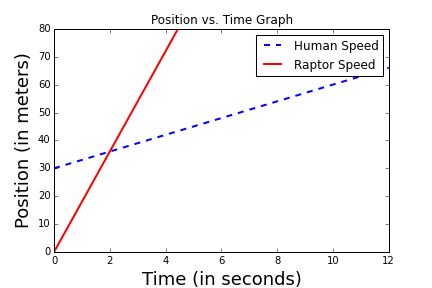
\includegraphics[width=0.5\textwidth]{CSISFinalProject1.png}
	\caption{Graph of Position vs. Time for a Human and a Raptor. \label{fig:Graph}}
\end{figure}

From the graph above, the point of intersection in the graph represented the point at which the raptor would catch the human. It was determined that the raptor would catch the human when the human ran six meters in two seconds. 
%%%%%%%%%%%%%%%%%%%%%%%%%%%%%%%%%%%%%%%%%%%%%%%%%%%%%%%%%%%%%%%%%%%%%%%%%%%%%%%%
\section{Question 3} 
The next question to answer was how far it would take the human to run when the raptor was one meter behind and the time it would have taken to be one meter behind. 

\begin{figure}[h]
	\centering
	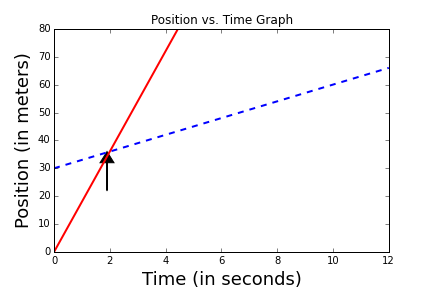
\includegraphics[width=0.5\textwidth]{CSISFinalProject2.png}
	\caption{A graph of Position versus Time with an arrow pointing at the place at which the raptor will be one meter behind.} \label{graph}
\end{figure}

Using a for loop and three empty lists for time, human distance and raptor distance, it was determined that after running 5.82 meters, the raptor would be one meter behind the human. Applying a for loop to return the first value of the result of a human's run minus a raptor's run that was lower then one gave me the answer as to how far the average human would have ran when the raptor was one meter behind. Time also got the same function and returned the time with which the raptor would be one meter behind. After running for 1.94 seconds, the raptor would be one meter behind the human. 
%%%%%%%%%%%%%%%%%%%%%%%%%%%%%%%%%%%%%%%%%%%%%%%%%%%%%%%%%%%%%%%%%%%%%%%%%%%%%%%%
\section{Question 4}

%%%%%%%%%%%%%%%%%%%%%%%%%%%%%%%%%%%%%%%%%%%%%%%%%%%%%%%%%%%%%%%%%%%%%%%%%%%%%%%%
In this question, I determined whether or not a human can survive three tries of a raptor trying to bite him. For the code, I started off by assigning three different variables to three random numbers that I let numpy choose for me. After naming the variables, I placed nested conditionals that would allow the program to determine whether or not the human got bit at any of the three tries which would mean immediate death. If at any of the times, the human got bit even once according to the possibility it could get bit, the program would stop there unless it survived the encounter. If the human survived the first encounter,  the program will continue to see if the raptor will have a better chance of catching the human, and a third time if the raptor is still yet unsuccessful. If the human survived all three encounters, he would yell "SWEET FREEDOM!" Testing this experiment with one thousand humans, the probability that humans would survive the encounters was around sixty-four percent.  
%%%%%%%%%%%%%%%%%%%%%%%%%%%%%%%%%%%%%%%%%%%%%%%%%%%%%%%%%%%%%%%%%%%%%%%%%%%%%%%%
%\section{Conclusion}
%%%%%%%%%%%%%%%%%%%%%%%%%%%%%%%%%%%%%%%%%%%%%%%%%%%%%%%%%%%%%%%%%%%%%%%%%%%%%%%%
%Based on the findings, it was concluded that in a experiment of one thousand trials, the raptor would h%ave around a sixty-four percent chance of biting a human. 

%%%%%%%%%%%%%%%%%%%%%%%%%%%%%%%%%%%%%%%%%%%%%%%%%%%%%%%%%%%%%%%%%%%%%%%%%%%%%%%%
\end{document}
%%%%%%%%%%%%%%%%%%%%%%%%%%%%%%%%%%%%%%%%%%%%%%%%%%%%%%%%%%%%%%%%%%%%%%%%%%%%%%%%
